\chapter{まえがき}
\label{chap:chap00-preface}
\begin{reviewimage}%%gmail
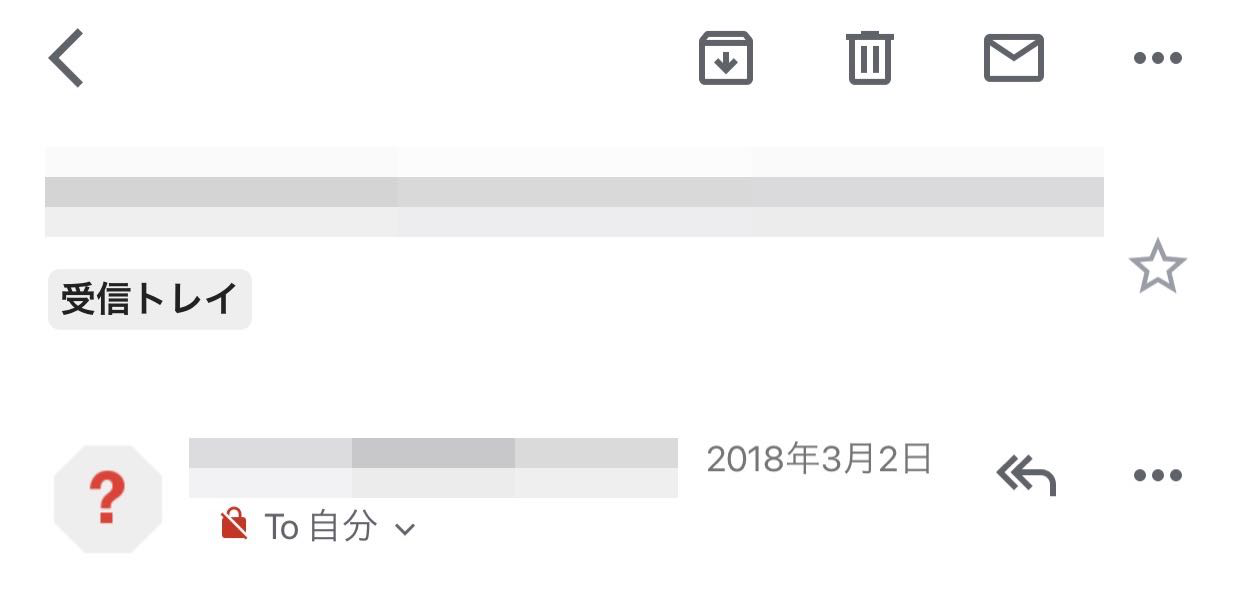
\includegraphics[width=\maxwidth]{./images/chap00-preface/gmail.png}%
\reviewimagecaption{Gmailに出てくる?マーク}
\label{image:chap00-preface:gmail}
\end{reviewimage}

Gmailにて、このようなメールが届いたことありますか?\\
または、試しに会社や取得したドメインで、ご自身のGmailアドレスメール送信してみてください。\\
Gmailで表示される?マークはスパムメールとして判定される前段階の状態、このまま放置しておくとスパムメールとしてメールが届かなくなります。この状態にならないため早めの対策が必要です。\\
これらの技術はSPF()とDKIM()によって行われます。SPFはメール送信する場所の正当性、DKIMは送信するメールサーバーの正当性を検証する技術になります。

本書は、メール送信で必要不可欠なSPFやDKIMの話を、わかりやすく解説した本です。この本を読めば、SPFやDKIMの基礎的なことが身につき送信するメールがスパムメールにされなくなります。

\paragraph*{本書で得られること}
\label{sec:-0-0-0-1}

\begin{itemize}
\item メール送信の正当性についての知識
\item SPFについての基礎的な知識
\item DKIMについての基礎的な知識
\item スパムメールにならないための設定知識
\end{itemize}

\paragraph*{対象読者}
\label{sec:-0-0-0-2}

\begin{itemize}
\item ドメインを取得したけど、メールを使っていない人
\item 会社のメールアドレスからメールを出しても、クライアントから届かないと言われて困っている人
\item フリーランスで仕事をはじめたけど、メールが届くか心配な人
\end{itemize}

\paragraph*{前提知識}
\label{sec:-0-0-0-3}

\begin{itemize}
\item メール配信の基本的な知識
\item ドメイン取得する知識
\item ドメイン設定を変更できるだけの知識
\item DNSに関する簡単な知識
\end{itemize}

\paragraph*{問い合わせ先}
\label{sec:-0-0-0-4}

\begin{itemize}
\item URL: https://sapi{-}kawahara.netlify.com/
\item Twitter: @sapi\textunderscore{}kawahara
\end{itemize}
